% !TeX TXS-program:compile = txs:///pdflatex/[-shell-escape]
% !TeX TXS-program:pdflatex = pdflatex -synctex=1 -interaction=nonstopmode --shell-escape %.tex
\section{Software Introspection}\label{sec:05_software_introspection}

\sectiontoc

\subsection{Disassembling Programs}\label{subsec:disassembling_programs}

Vamos a usar unas de las herramientas más comunes, que es \mintinline{bash}{objdump}, y se usará las siguientes banderas de ejecución:

\begin{itemize}
	\item \mintinline{bash}{-d}: Para que haga un disassembling, de las secciones que tiene instrucciones de ensamblador.
	\item \mintinline{bash}{-M intel}: Es para escoger la sintaxis a la cual le vamos a realizar disassembling.
\end{itemize}

\begin{codebox}[bash]{}
	objdump -d -M intel /tmp/your_program
\end{codebox}

Y vamos a tener una salida similar a esta de aquí:

\begin{codebox}[bash]{}
	hacker@dojo:~$ objdump -d -M intel /tmp/your-program

	/tmp/your-program:     file format elf64-x86-64


	Disassembly of section .text:

	0000000000401000 <_start>:
	401000: 48 c7 c7 39 05 00 00  mov    rdi,0x539
	401007: 48 c7 c7 00 00 00 00  mov    rdi,0
	40100e: 48 c7 c0 3c 00 00 00  mov    rax,0x3c
	401015: 0f 05                 syscall
\end{codebox}

\begin{figure}[!ht]
	\centering
	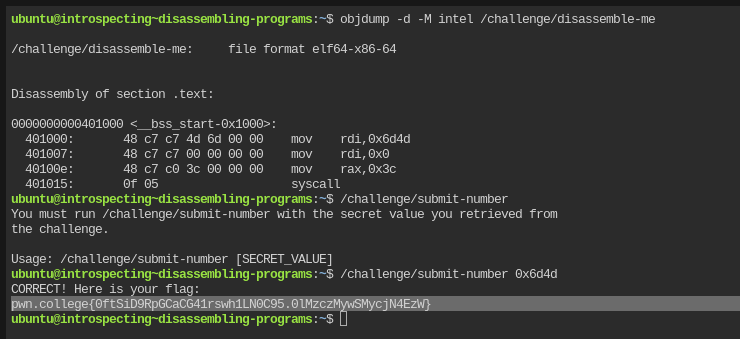
\includegraphics[width=0.8\textwidth]{img/05_software_introspection/disassembling_programs.png}
	\caption{Disassembling Programs Result}
\end{figure}

\subsection{Tracing Syscalls}\label{subsec:tracing_syscalls}

Con el programa \mintinline{bash}{strace} nos permite poder ver las llamadas a syscall, que
realiza un programa.

\begin{codebox}[bash]{}
	hacker@dojo:~$ strace /tmp/your-program
		execve("/tmp/your-program", ["/tmp/your-program"], 0x7ffd48ae28b0 /* 53 vars */) = 0
		exit(42)                                         = ?
		+++ exited with 42 +++
		hacker@dojo:~$
\end{codebox}

En este caso, vemos que al momento de ejecutar \mintinline{bash}{strace}, nos muestra la
ejecución de los syscall, en un formato parecido a las funciones en C.

\begin{codebox}[C]{}
	system_call(parameter, parameter, parameter, ... )
\end{codebox}

Donde los \mintinline{C}{parameter} son los valores que se le manda a ejecutar.

\subsection{Starting GDB}\label{subsec:starting_gdb}

GDB = GNU Debugger

Ejecución del GDB:

\begin{codebox}[bash]{}
	gdb /path/to/file
\end{codebox}

\subsection{Quitting GDB}\label{subsec:quitting_gdb}

Para salir del GDB, tenemos que escribir quit, o q.

\subsection{Starting Programs in GDB}\label{subsec:starting_programs_in_gdb}

Con el comando \mintinline{bash}{starti} en GDB, se indica que el programa empiece a ejecutarse,
desde la línea de código, y vamos a poder ver su comportamiento, en tiempo
de ejecución.

Por ejemplo, vamos a poder desensamblar el programa con \mintinline{bash}{disassemble}.

\subsection{Disassembling in GDB}\label{subsec:disassembling_in_gdb}

Lo mismo que el código pasado, no entender el porqué, pero bueno.

\subsection{Stepping Through Instructions}\label{subsec:stepping_through_instructions}

Podemos realizar la ejecución paso a paso, con \mintinline{bash}{stepi}, o usando la versión corta con \mintinline{bash}{si}.

\subsection{Reading Register Values}\label{subsec:reading_register_values}

\subsection{Setting Register Values}\label{subsec:setting_register_values}

\subsection{Popping Stack Values}\label{subsec:popping_stack_values}

\subsection{Examining Memory}\label{subsec:examining_memory}

\subsection{Examining Stack Pointers}\label{subsec:examining_stack_pointers}

\subsection{Cooperate Debugging}\label{subsec:cooperate_debugging}

\subsection{Running with Arguments}\label{subsec:running_with_arguments}

\subsection{Redirecting Input in GDB}\label{subsec:redirecting_input_in_gdb}
